\documentclass{beamer}

\usepackage{cmap} % для кодировки шрифтов в pdf
\usepackage[utf8x]{inputenc}
\usepackage[russian]{babel}
\usepackage[T1,T2A]{fontenc}
\usepackage{beamerthemesplit}
\usepackage{algorithm}
\usepackage{algpseudocode}
\usepackage{graphics,epsfig, subfigure}
\usepackage{url}

\definecolor{kugreen}{RGB}{50,93,61}
\definecolor{kugreenlys}{RGB}{132,158,139}
\definecolor{kugreenlyslys}{RGB}{173,190,177}
\definecolor{kugreenlyslyslys}{RGB}{214,223,216}
\setbeamercovered{transparent}
\mode<presentation>
{    \usetheme{Warsaw}
  \usecolortheme[named=kugreen]{structure}
\useinnertheme{circles}
\usefonttheme[onlymath]{serif}
\setbeamercovered{transparent}
\setbeamertemplate{blocks}[rounded][shadow=true]
\setbeamertemplate{footline}[page number]{}
}
%\setbeamertemplate{background}{\includegraphics[width=1\textwidth]{natfak_baggrund.pdf}}
% \logo{\includegraphics[width=1cm]{billeder/logo}}

\title{Разработка алгоритмов оптимизации групповой работы мобильных роботов}
\author{Студент группы с8503а, Спорышев М. С.}
\institute{Руководитель: \\ н.с. лаборатории необитаемых подводных аппаратов и их систем, к.т.н. Туфанов И. Е.}
\date{25 Июня 2015}


\begin{document}

\begin{frame}[noframenumbering]
\titlepage

\end{frame}

% ituphanov
% Общее замечание по презенташке: шрифты маловаты. Например, на слайде "перепланирование"
% где-то посередине надпись и всё пространство вокруг свободно.
% В бимере это пофиксить сложновато, но если получится - будет хорошо.
% Хотя, есть слайды насыщенные текстом и их не пофиксишь.

% ituphanov
% Общее замечание. Мне кажется, введение получается слишком растянутым,
% поэтому я за то, чтобы эти слайды скомпановать.

% ituphanov
% Общее замечание. презентацию можно распечатать по 2 слайда на листе 
% экземплярах в 5-7 и выдать членам комиссии как раздаточный материал.
% Тогда они его будут листать и тебя вообще слушать не будут.

% ituphanov
% Потренируй доклад. Если не будет времени на этот слайд, то пролистни его, а в раздатке пусть будет.
% Когда тренируешься, не говори быстро.
\begin{frame}{Термины}
\begin{itemize}
\item АНПА -- автономный необитаемый подводный аппарат
\item СПУ -- система программного управления
\item ГА -- генетический алгоритм
\end{itemize}
\end{frame}

% ituphanov
% Вот на этот слайд подошла бы картника с аппаратом, которая у тебя ниже
\begin{frame}{Автономные необитаемые подводные аппараты}

 \begin{columns}[onlytextwidth, t]
    \begin{column}{0.5\textwidth}

        Обзорно-поисковые задачи
        \begin{itemize}
        \item Поиск затонувших объектов
        \item Замеры параметров водной среды
        \item Исследование локальных неоднородностей
        \end{itemize}
    \end{column}
% ituphanov
% Было бы хорошо между колонками вставить зазор, а то текст налезает.
    \begin{column}{0.5\textwidth}

        Использование групп АНПА
        \begin{itemize}
        \item Централизованное управление
        \item Групповое управление
        \end{itemize}

    \end{column}

​\end{columns}



\end{frame}

% ituphanov
% Я не сразу понял, что этот слайд как бы анонсирует три следующих и они тоже связаны.
% Обычно, если есть такой ход в сюжете доклада, то никто не успевает следить за этим.
% Например, если слушатель пропустит вот этот слайд, он упустит связь между тремя последующими.
% Надо или придумать как их специально пометить (например, на каждом слайде рисовать сверху эти
% три пункта серым, а текущий отмечать чёрным), или, что мне больше нравится,
% объединить в один, выкинув лишние слова.
% Отступление. Репплан говорит, что нужно 10-15 слов на слайде. Я с этим не согласен.
% Тем более, твой шрифт позволяет сделать больше. Если на слайде мало слов, то будет много 
% слайдов и ты их будешь часто перелистывать, не давая слушателю вообще понять что происходит.
% Даже внимательный слушатель от тебя остаёт. Или сначала читает слайд, потом слушает тебя, потом 
% ещё раз читает. Если ты будешь слайды держать по 10-20 секунд, он вообще ничего не поймёт.
\begin{frame}{Используемая система управления}

\begin{enumerate}
\item Составление заданий для аппаратов
\item Распределение заданий между аппаратами

\item Перепланирование


\end{enumerate}
\end{frame}

% ituphanov
% Я за то чтобы объединить следующие три слайда (а предыдущий выкинуть), 
% под заголовком типа "Задача оптимизации плана"). Картника хорошая, она всё поясняет.
% Может быть, её стоит перегенерить, сделав цвета ярче, потому что проектор сделает их одинаковыми.
% Нужен ярко-синий и ярко-зелёный. И Кружочки не должны быть синими. Пусть лучше серыми.
% Если подписать на картнике s_1, s_2, a_11, b_11, ... (при этом концы заданий получат по 2 обозначения),
% то это может быть вообще вин, все всё поймут.
% Текст оставить только важный. У тебя, например, 3 строки написано про то, что каждое задание надо
% вополнить в одном варианте и т.д., но нигде не сказано, что ты решаешь задачу оптимизации.
% В общем, здесь если подумать, то можно сделать хорошо.
\begin{frame}{Составление заданий для аппаратов}
Составляются $n$ заданий. Предполагается, что каждый аппарат может выполнять каждое задание.
\begin{columns}[onlytextwidth, t]
    \begin{column}{0.6\textwidth}

        $i$--e задание может быть выполнено в одном из $v_i$ вариантов:
        \begin{itemize}
        \item $(\mathbf{a_{i 1}}, \mathbf{b_{i 1}}, \tau_{i 1})$
        \item $(\mathbf{a_{i 2}}, \mathbf{b_{i 2}}, \tau_{i 2})$
        \item $...$
        \item $(\mathbf{a_{i v_i}}, \mathbf{b_{i v_i}}, \tau_{i v_i})$
        \end{itemize}

    \end{column}
    \begin{column}{0.4\textwidth}
% ituphanov
% вот эту картинку я предлагаю наверх.
        \begin{figure}[here]
            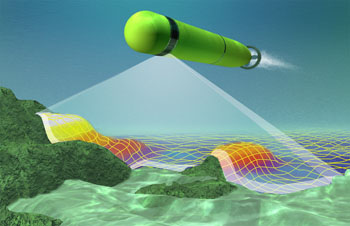
\includegraphics[scale=0.4]{images/AUV5.JPG}
        \end{figure}
    \end{column}

​\end{columns}
\end{frame}

\begin{frame}{Распределение заданий между аппаратами}
Имеется $m$ аппаратов. Каждому аппарату составляется план заданий так, чтобы каждое было выполнено в единственном варианте, только одним аппаратом, единственный раз.
\begin{columns}[onlytextwidth, t]
    \begin{column}{0.6\textwidth}
        \linebreak
        Результат распределения заданий:
        \begin{itemize}
            \item $q$--му аппарату соответствует последовательность пар номеров заданий и их вариантов:
            $p_q = ((i_1, j_1), (i_2, j_2), ..., (i_{|p|}, j_{|p|}))$
            \item $\forall k \in 1..|p|~ $
            \begin{itemize}
                \item $i_k \in 1..n$ -- номер задания
                \item $j_k \in 1..v_{i_k}$  -- номер варианта
            \end{itemize}

        \end{itemize}

    \end{column}
    \begin{column}{0.4\textwidth}

        \begin{figure}[here]
            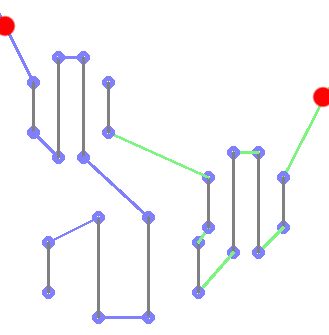
\includegraphics[scale=0.4]{images/hk2.png}
        \end{figure}
    \end{column}

​\end{columns}
\end{frame}

\begin{frame}{Перепланирование}
\begin{itemize}
\item Выход аппарата из строя
\item Появление нового аппарата
\item Появление новых заданий
\item Изменение заданий
\end{itemize}
\end{frame}

% ituphanov
% Основная задача этого слайда - постановка цели, я предлагаю поменять заголовок.
% А то что у тебя написано для ХК, написать типа "Раньше использовался алгоритм Хельда-Карпа:"
\begin{frame}{Использующийся алгоритм}

Алгоритм Хельда-Карпа
\begin{itemize}
\item Экспоненциальная зависимость времени работы от количества заданий (Перебор подмножеств)
\item Работает дольше минуты для 20 заданий
\end{itemize}

% ituphanov
% Как мы выясняли с Клениным, до минуты, это слишком круто. Я бы сказал, "порядка нескольких минут".
\begin{block}{Цель}
Разработать новые алгоритмы для решения задачи планирования, способные составлять планы для 100 заданий и 5 аппаратов за приемлемое время(до минуты) и внедрить их в существующую СПУ.
\end{block}

\end{frame}

% ituphanov
% Во. Вот этот слайд, можно убрать отсюда и частично использовать выше.
% Потому что у тебя как бы в обоих слайдах речь идёт об одном и том же.
% Можно сделать слайд "Задача оптимизации плана".
\begin{frame}{Математическая модель}


\begin{block}{Входные данные}
\begin{itemize}
\item Имеется $m$ аппаратов и $n$ заданий. $q$-ый аппарат в начальный момент времени находится в точке $s_q$
\item $d_q(\mathbf{a}, \mathbf{b}) = |\mathbf{a} - \mathbf{b}| / u_q$ ~-- время перехода АНПА от точки $\mathbf{a}$ к точке $\mathbf{b}$, где $u_q$ - максимальная скорость $q$-го аппарата.
\end{itemize}
\end{block}

\begin{itemize}

\item План $q$-го аппарата: $p = ((i_1, j_1), (i_2, j_2), ..., (i_{|p|}, j_{|p|}))$.

\item
$
t_q(p) = d_q(\mathbf{s}_q, \mathbf{a}_{i_1, j_1}) + \displaystyle\sum_{k=2}^{|p|} d_q(\mathbf{b}_{i_{k-1} j_{k - 1}}, \mathbf{a}_{i_k j_k}) + \displaystyle\sum_{k=1}^{|p|}\tau_{i_k j_k}
$

\item Общий план $P = (p_1, p_2, ..., p_m)$
\item Время выполнения общего плана: $t(P) = \displaystyle \max_{q \in 1..m} t_q(p)$

\end{itemize}

\begin{block}{Задача}
Найти общий план $P$, при котором $t(P) \rightarrow \min$
\end{block}

\end{frame}

\begin{frame}{Существующие решения}
\begin{columns}[onlytextwidth, t]
    \begin{column}{0.6\textwidth}
        Множественная задача коммивояжера
        \begin{itemize}
        \item Каждое задание является единственной точкой
        \item Полный граф
        \item Стартовая вершина
        \item Поиск оптимальной системы циклов
% ituphanov
% суммы, максимума -> суммы или максимума
        \item Минимизация суммы, максимума
        \end{itemize}

    \end{column}
    \begin{column}{0.4\textwidth}

        \begin{figure}[here]
            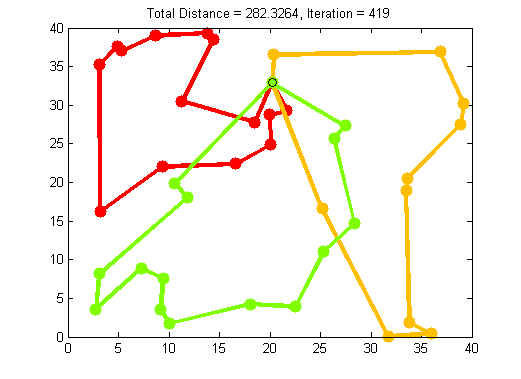
\includegraphics[scale=0.4]{images/mtsp.png}
        \end{figure}
    \end{column}

​\end{columns}

\end{frame}

\begin{frame}{Жадный алгоритм}
% \begin{algorithm}
% \floatname{algorithm}{Алгоритм}
% \caption{Жадный алгоритм}\label{alg:greedy}
\begin{algorithmic}[1]

\ForAll {$t \in T$}
    \ForAll {$var \in Vars(t)$}
        \ForAll {$v \in V$}
            \State $time, pos \gets$ \Call{MinPathTime}{$t, var, Plan(v)}$
            \If {$time < minTime$}
                \State $minTime \gets time$
                \State $bestPos \gets pos$
                \State $bestV \gets v$
                \State $bestVar \gets var$
            \EndIf
        \EndFor
    \EndFor
    \State \Call{Insert}{$t, bestVar, Plan(bestV), bestPos$}
    \State \Call{OptimizeVars}{$bestV$}
\EndFor

\end{algorithmic}
% \end{algorithm}

\end{frame}

% ituphanov
% Наверное, его надо вставить перед жадником, потому что он как бы между жадником и ГА,
% и используется и там и там.
\begin{frame}{Оптимальный выбор вариантов}
Известен план некоторого аппарата, найти варианты заданий, дающие минимальное время выполнения этого плана.

Метод динамического программирования
\begin{itemize}
\item Номер последнего задания
\item Номер варианта задания
\end{itemize}

\begin{exampleblock}{Переход к следующему состоянию}

\begin{algorithmic}
\State $val \gets d[i - 1][var1] + Dist(v, p[i - 1], var1, p[i], var2)$
\If {$d[i][var2] > val$}
    \State $d[i][var2] \gets Min(d[i][var2], val)$
    \State $prev[i][var2] = var1$
\EndIf
\end{algorithmic}

\end{exampleblock}

\end{frame}

% ituphanov
% Вот здесь у тебя набор ключевых слов. Может быть, стоит что-то добавить.
% Например, ты пишешь "Функция приспособленности", но это толко подлежащее. 
% Читатель спросит: "что функция приспособленности?", если прослушает пару твоих слов,
% а прослушает он обязательно.
\begin{frame}{Генетический алгоритм}
\begin{columns}[onlytextwidth]
    \begin{column}{0.6\textwidth}
        \begin{itemize}
            \item Решение представлено в виде двух хромосом
            \begin{itemize}
            \item Перестановка номеров заданий
            \item Последовательность номеров аппаратов
            \end{itemize}

            \item 3 вида мутаций
            \begin{itemize}
            \item Swap
            \item Reverse
            \item Select
            \end{itemize}

            \item Скрещивание -- Partially matched crossover
            \item Функция приспособленности
        \end{itemize}

    \end{column}
    \begin{column}{0.4\textwidth}

        \begin{figure}[here]
            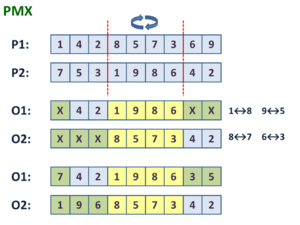
\includegraphics[scale=0.5]{images/300px-Pmx.png}
        \end{figure}
    \end{column}

​\end{columns}
\end{frame}

% ituphanov
% Вот здесь пункты 2 и 4 сформулированы так, что кажутся противоречащими друг другу.
% Надо их разнести к разным перечислениям. Например:
% 
% Почему именно этот подход?
% - Обеспечивает точное решение
% - Позволяет решить задачу коммивояжёра для m = 100 за секунды
% Реализация:
% - решение строится для упрощённой задачи
% - использование библиотеки SYMPHONY для метода ветвей и границ
% - минимизация максимума через минимизацию суммы с доп. ограничениями
% - уступает алгоритму Хельда-Карпа по времени вычислений
\begin{frame}{Целочисленное программирование}
\begin{itemize}
\item Точное решение
\item TSP -- сотни заданий за секунды
\item Множественная задача коммивояжера
    \begin{itemize}
    \item Оптимизация максимума
    \item Бинарный поиск максимума и оптимизация суммы с доп. ограничениями
    \end{itemize}

\item Работает медленнее алгоритма Хельда-Карпа
\end{itemize}
\end{frame}

\begin{frame}{Реализация}

% ituphanov
% Вставь пару слов про то, для чего использовалась каждая библиотека:
% OpenCV~--- визуализация полученных решений
Стороннине библиотеки
\begin{itemize}
\item FlopC++
\item SYMPHONY
\item OpenCV
\item Boost
\end{itemize}

Python
\begin{itemize}
\item Pandas
\item matplotlib
\end{itemize}

\end{frame}

\begin{frame}{Тестирование}
Визуализация
\begin{figure}[here]
    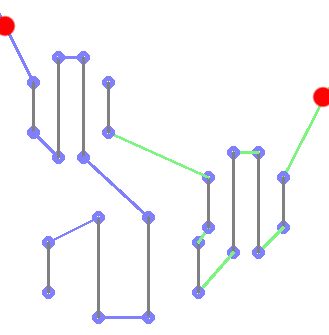
\includegraphics[scale=0.5]{images/hk2.png}
\end{figure}

\end{frame}


\begin{frame}{Тестирование}
Время выполнения плана на каждом тесте
\begin{figure}[here]
    \includegraphics[scale=0.5]{images/test_small1.jpg}
\end{figure}

\end{frame}


% ituphanov
% Не видно будет ничего. Надо как минимум растянуть картинку до предела.
% Как максимум: перегенерить, сделав шрифты крупнее.
\begin{frame}{Тестирование}
Стоимость решения ГА от количества итераций
\begin{figure}[here]
    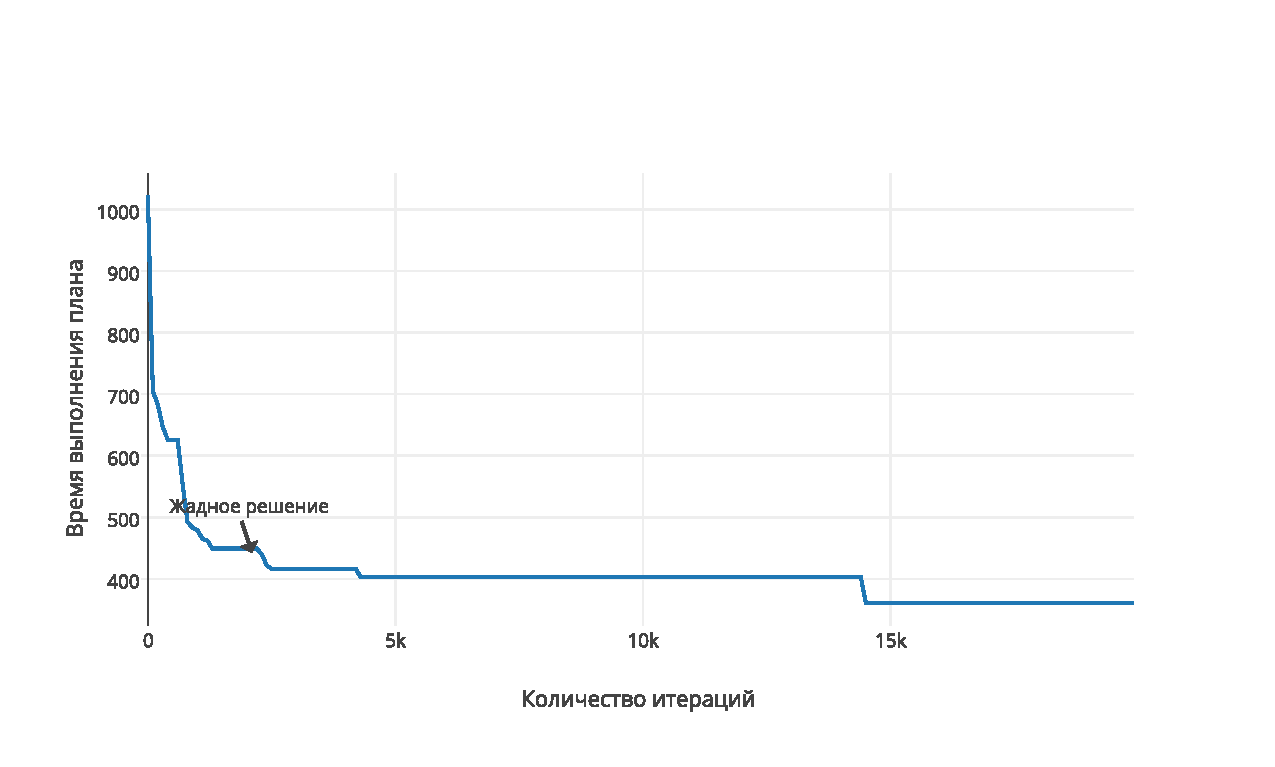
\includegraphics[scale=0.5]{images/iter-value-20-plot.eps}
\end{figure}

\end{frame}

% ituphanov
% Странно было бы, если бы был оборот "неуспешно внедрены".
% Я предлагаю "Алгоримы внедрены в СПУ комплекса "МАРК"". А можно ещё и фотку.
% Ещё накинь пару слов: "Автоматический выбор алгоритма в зависимости от размера задачи:"
% Ты проверил, что group_controller не падает?
% Запросто могут спросить: "Как вы проверили, что внедрены успешно? Ведь аппараты в воде не плавали."
% я бы вообще объединил со следующим слайдом.
\begin{frame}{Результат}
Алгоритмы успешно внедрены
\begin{itemize}
\item до 18 заданий -- алгоритм Хельда-Карпа
\item до 40 заданий -- генетический алгоритм
\item от 40 заданий -- жадный алгоритм
\end{itemize}
\end{frame}

\begin{frame}{Заключение}
\begin{itemize}
\item Система контроля версий git, 52 коммита, +4900 -1800. Языки C++ и Python.
\end{itemize}

\end{frame}

\end{document}
